\documentclass[11pt]{article}
\usepackage{graphicx}
\usepackage{hyperref}
\usepackage{amsmath}
\usepackage{amsthm}
\usepackage{amssymb}
\usepackage[all=normal,floats,leading,paragraphs,charwidths,tracking,wordspacing]{savetrees}
\usepackage{float}
%\usepackage[version = 4]{mhchem}
\usepackage{multirow}
\usepackage{commath}
\usepackage{booktabs}
\usepackage{adjustbox}
\usepackage{subcaption}
\usepackage{rotating}
\usepackage{natbib}
%\renewcommand{\arraystretch}{1.2}
\usepackage[nottoc,numbib]{tocbibind}
\usepackage{siunitx}
\sisetup{detect-all}
\DeclareSIUnit{\atm}{atm}
\usepackage{listings}
\usepackage{color} %red, green, blue, yellow, cyan, magenta, black, white
\definecolor{mygreen}{RGB}{28,172,0} % color values Red, Green, Blue
\definecolor{mylilas}{RGB}{170,55,241}
\usepackage[a4paper,margin=20mm]{geometry}
%\numberwithin{equation}{section}
\setlength{\parskip}{\baselineskip}
\setlength{\parindent}{0pt}
\NewDocumentCommand\Pounds{o}{%
\pounds\IfNoValueTF{#1}%
{\relax}{\,\num[]{#1}}}
\hypersetup{
    colorlinks=true,
    linkcolor=black,
    filecolor=black,      
    urlcolor=black,
    citecolor=black
}
\urlstyle{same}
\lstset{language=Matlab,%
    %basicstyle=\color{red},
    breaklines=true,%
    morekeywords={matlab2tikz},
    keywordstyle=\color{blue},%
    morekeywords=[2]{1}, keywordstyle=[2]{\color{black}},
    identifierstyle=\color{black},%
    stringstyle=\color{mylilas},
    commentstyle=\color{mygreen},%
    showstringspaces=false,%without this there will be a symbol in the places where there is a space
    numbers=left,%
    numberstyle={\tiny \color{black}},% size of the numbers
    numbersep=9pt, % this defines how far the numbers are from the text
    emph=[1]{for,end,break},emphstyle=[1]\color{red}, %some words to emphasise
    %emph=[2]{word1,word2}, emphstyle=[2]{style},    
}
\begin{document}
\begin{titlepage}
    \begin{center}
        \vspace*{1cm}
             
        MSIN0068 Project Management\\
        2021/22
 
        \vspace{1.5cm}

        {\LARGE \textbf{Individual Coursework} \par}
             
        \vspace{1.5cm}
 
        Anonymous
        
        \vfill

        University College London\\
        Torrington Place\\
        LONDON WC1E 7JE
             
    \end{center}
 \end{titlepage}
\newpage
\section*{Question A1}
\begin{figure}[H]
    \centering
    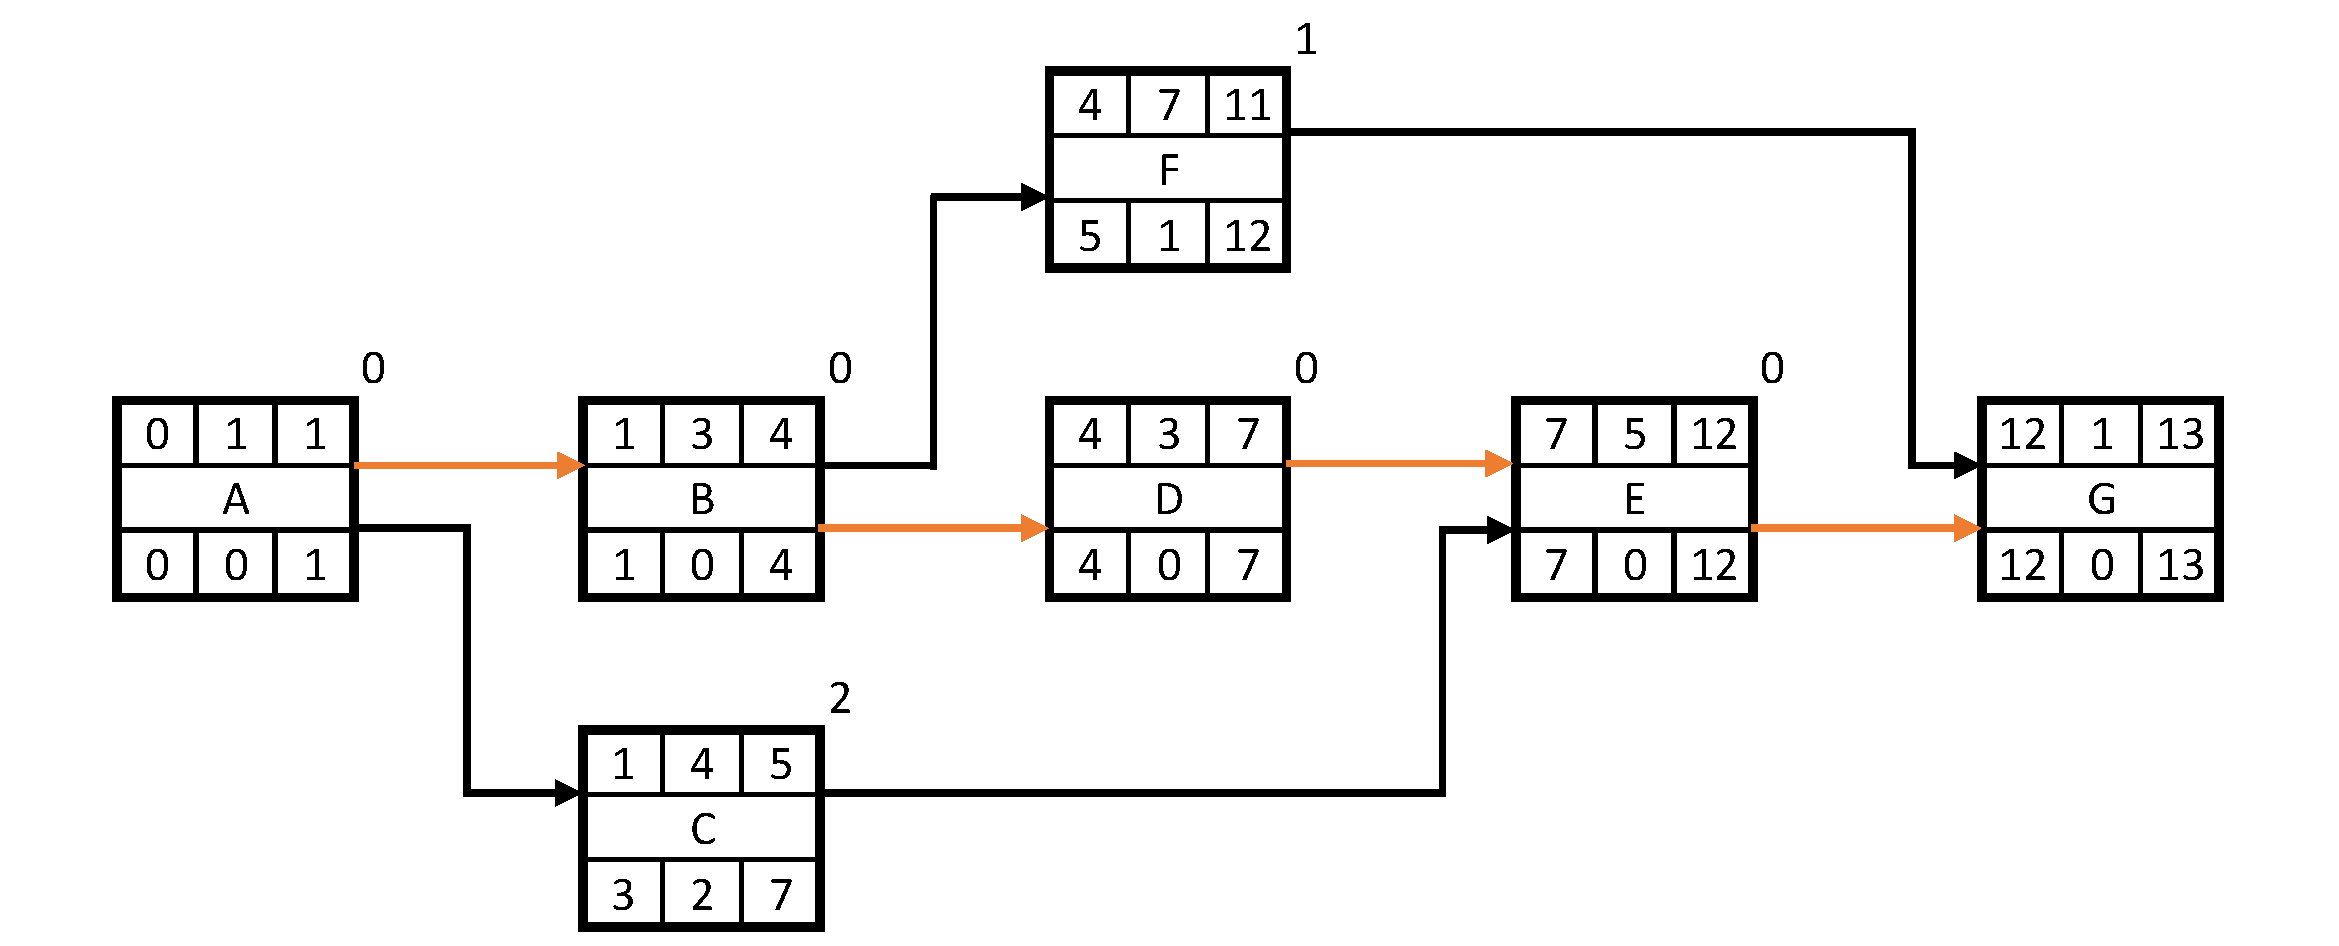
\includegraphics[width = \textwidth]{./img/qa1.png}
    \caption{Network diagram to show `normal' project timescale.}
    \label{qa1}
\end{figure}
From Figure \ref{qa1}, we can see the project duration is 13 days with the critical load path highlighted in orange. 
\section*{Question A2}
We can find out the values for our cost/time slop by utilising the following:
\begin{equation}
    \frac{\Delta_c}{\Delta_d}
\end{equation}
where $\Delta_c$ is the difference between the normal and crash costs and $\Delta_d$ is the difference between the normal and crash durations.
\begin{table}[H]
    \centering
    \begin{tabular}{@{}
        l
        S[table-format= 4  ,table-number-alignment=left]
        S[table-format= 5  ,table-number-alignment=left]
        S[table-format= 4  ,table-number-alignment=left]
        S[table-format= 1  ,table-number-alignment=left]
        S[table-format= 1  ,table-number-alignment=left]
        S[table-format= 1  ,table-number-alignment=left]
        S[table-format= 4  ,table-number-alignment=left]
        @{}}
        \toprule
        & \multicolumn{3}{l}{Cost (£)} & \multicolumn{3}{l}{Duration (days)} & \\
        \midrule
        \multirow{2}{*}{Activity} & {\multirow{2}{*}{Normal}} & {\multirow{2}{*}{Crash}} & {\multirow{2}{*}{$\Delta_{c}$}} & {\multirow{2}{*}{Normal}} & {\multirow{2}{*}{Crash}} & {\multirow{2}{*}{$\Delta_{d}$}} & {Cost/time slope}\\
        & & & & & & & \multicolumn{1}{l}{($\Delta_{c}/\Delta_{d}$)} \\
        \midrule
        A & 1000 & 1000 & 0 & 1 & 1 & 0 & 0\\
        B & 4000 & 8000 & 4000 & 3 & 1 & 2 & 2000\\
        C & 5000 & 8000 & 3000 & 4 & 2 & 2 & 1500\\
        D & 3000 & 4000 & 1000 & 3 & 2 & 1 & 1000\\
        E & 6000 & 10000 & 4000 & 5 & 3 & 2 & 2000\\
        F & 7000 & 8000 & 1000 & 7 & 6 & 1 & 1000\\
        G & 2000 & 2000 & 0 & 1 & 1 & 0 & 0\\
        \bottomrule
    \end{tabular}
    \caption{Table to show cost/time slope for activities.}
    \label{qa2}
\end{table}
\newpage
\section*{Question A3}
The agreed contract price is \Pounds[52000] upon delivery (at full payment). Currently, the project will take 13 days to complete, which will incur a late penalty of \Pounds[5000] (late by two days - penalty of \Pounds[2500] per day). The projected cost of the normal timescale is \Pounds[28000]. Hence, after penalties and costs, our final profit will be \Pounds[19000]. However, this timescale is undesirable due to the late delivery of the project. This will impact the Remus' reputation with Nestbury, as it is highly likely that Nestbury would seek other firms for future business if the project is delivered late. Nestbury have requested for the timescale of the project to be reduced, `preferably to the shortest possible time'. We can ascertain that a reduction in timescale below the 11 day deadline is desirable. Therefore, it will be necessary to crash certain parts of the timescale. From Figure \ref{qa1}, there are two days of free float for activity C and 1 day of free float for activity F. To decide how to crash the project timescale, we can analyse the timescale using the least-cost method and by crashing the shortest activities.

From Table \ref{qa2}, we can see that crashing activity D will incur the least cost to Remus. This will reduce our timescale down to 12 days. We also find that activity F has been added the critical path (i.e. there are now two branches of the critical path). Our final profit value will increase to \Pounds[20500] but the project will still be delivered late, incurring both a penalty and reputational risk. This is represented as Option 1 in Table \ref{qa3-1}.

To further reduce our timescale, we must crash other activities. From Figure \ref{qa1} and least-cost analysis, crashing activity E (subsequently requiring us to crash F) is the next option. As we can crash activity E incrementally, we can choose to crash E by two days and F by one day. This will reduce the timescale to 11 days and result in a profit of \Pounds[19000]. This solution produces less profit but achieves the minimum timescale. This may also be seen as risky as any delays will push the project delivery date, incurring penalties. This can be seen as the `bare minimum' option and may not leave Nestbury with the feeling that Remus' will go above and beyond for them. This is represented as Option 2 in Table \ref{qa3-1}.

Finally, in order to reduce the timescale as much as possible, we can crash activities B, C, D, E and F. This option is the most expensive but reduces the timescale to 9 days. Our profit would be significantly reduced to \Pounds[11000] and delivering the project early would simply would be an act to impress Nestbury with our ability to produce work quickly (as there is no early delivery bonus). This option would add additional stress to the team and would require that freelancers are available and willing to take on the additional work (which may not be the case). There are also no free floats, hence a delay in any activity would cascade through the timescale and push the delivery date (for which there is two days of leeway). This is represented as Option 3 in Table \ref{qa3-1}.

Let us analyse the reduction of the timescale by crashing the shortest tasks. We can begin by crashing activity B. This will reduce the timescale to 11 days. However as mentioned previously this option may be seen as a `bare minimum'. This is represented as Option 4 in Table \ref{qa3-2}. We can further reduce the timescale by crashing activity E by one day, bringing our timescale down to ten days. This option also produces a profit of \Pounds[18000]. Delivering the project a day early will be received warmly by Nestbury and further our reputation with them for going above and beyond. 

To conclude, if we want to deliver the project on time, we can see that we achieve more profit with Option 4 versus Option 2, making it the better option of the two. In order to secure Nestbury as a long term client, we should impress the client by going above and beyond. Option 5 delivers the project early whilst sustaining average profit. Option 3 overly stresses the team and requires freelancers able to work the extra hours. Analysis shows us that crashing Option 5 also requires crashing only two tasks, whereas Option 3 requires crashing five tasks to shave one day off the timescale (with significant reduction in profit) - a diminished return. Despite all blocks being on the critical path in Option 5, we still have one day leeway for any delays. Hence, it would be in the best interest for Remus' to utilise Option 5, decreasing profit slightly at the benefit of securing Nestbury as a long-term client.

\begin{table}[H]
    \centering
    \begin{adjustbox}{max width=\textwidth}
    \begin{tabular}{@{}llllllllll@{}}
        \toprule
        & \multicolumn{3}{l}{Option 1} & \multicolumn{3}{l}{Option 2} & \multicolumn{3}{l}{Option 3}\\
        \midrule
        Activity & Days saved & Duration & Free float & Days saved & Duration & Free float & Days saved & Duration & Free float\\
        \midrule
        A & 0 & 1 & 0 & 0 & 1 & 0 & 0 & 1 & 0 \\
        B & 0 & 3 & 0 & 0 & 3 & 0 & 2 & 1 & 0 \\
        C & 0 & 4 & 1 & 0 & 4 & 2 & 1 & 3 & 0 \\
        D & 1 & 2 & 0 & 0 & 3 & 0 & 1 & 2 & 0 \\
        E & 0 & 5 & 0 & 2 & 3 & 0 & 2 & 4 & 0 \\
        F & 0 & 7 & 0 & 1 & 6 & 0 & 1 & 6 & 0 \\
        G & 0 & 1 & 0 & 0 & 1 & 0 & 0 & 1 & 0 \\
        \midrule
        Extra cost & \Pounds[1000] & & & \Pounds[5000] & & & \Pounds[13000] & & \\
        Penalties & \Pounds[2500] & & & \Pounds[0] & & & \Pounds[0] & & \\
        Duration & 12 days & & & 11 days & & & 9 days & & \\
        Profit & \Pounds[20500] & & & \Pounds[19000] & & & \Pounds[11000] & & \\
        \bottomrule
    \end{tabular}
    \end{adjustbox}
    \caption{Table to show least-cost crashing analysis.}
    \label{qa3-1}
\end{table}

\begin{table}[H]
    \centering
    \begin{adjustbox}{max width=\textwidth}
    \begin{tabular}{@{}lllllll@{}}
        \toprule
        & \multicolumn{3}{l}{Option 4} & \multicolumn{3}{l}{Option 5}\\
        \midrule
        Activity & Days saved & Duration & Free float & Days saved & Duration & Free float \\
        \midrule
        A & 0 & 1 & 0 & 0 & 1 & 0 \\
        B & 2 & 1 & 0 & 2 & 1 & 0 \\
        C & 0 & 4 & 0 & 0 & 4 & 0 \\
        D & 0 & 3 & 0 & 0 & 3 & 0 \\
        E & 0 & 5 & 0 & 1 & 4 & 0 \\
        F & 0 & 7 & 1 & 0 & 7 & 0 \\
        G & 0 & 1 & 0 & 0 & 1 & 0 \\
        \midrule
        Extra cost & \Pounds[4000] & & & \Pounds[6000] & & \\
        Penalties & \Pounds[0] & & & \Pounds[0] & & \\
        Duration & 11 days & & & 10 days & & \\
        Profit & \Pounds[20000] & & & \Pounds[18000] & & \\
        \bottomrule
    \end{tabular}
    \end{adjustbox}
    \caption{Table to show shortest task crashing.}
    \label{qa3-2}
\end{table}
\section*{Question A4}
\begin{figure}[H]
    \centering
    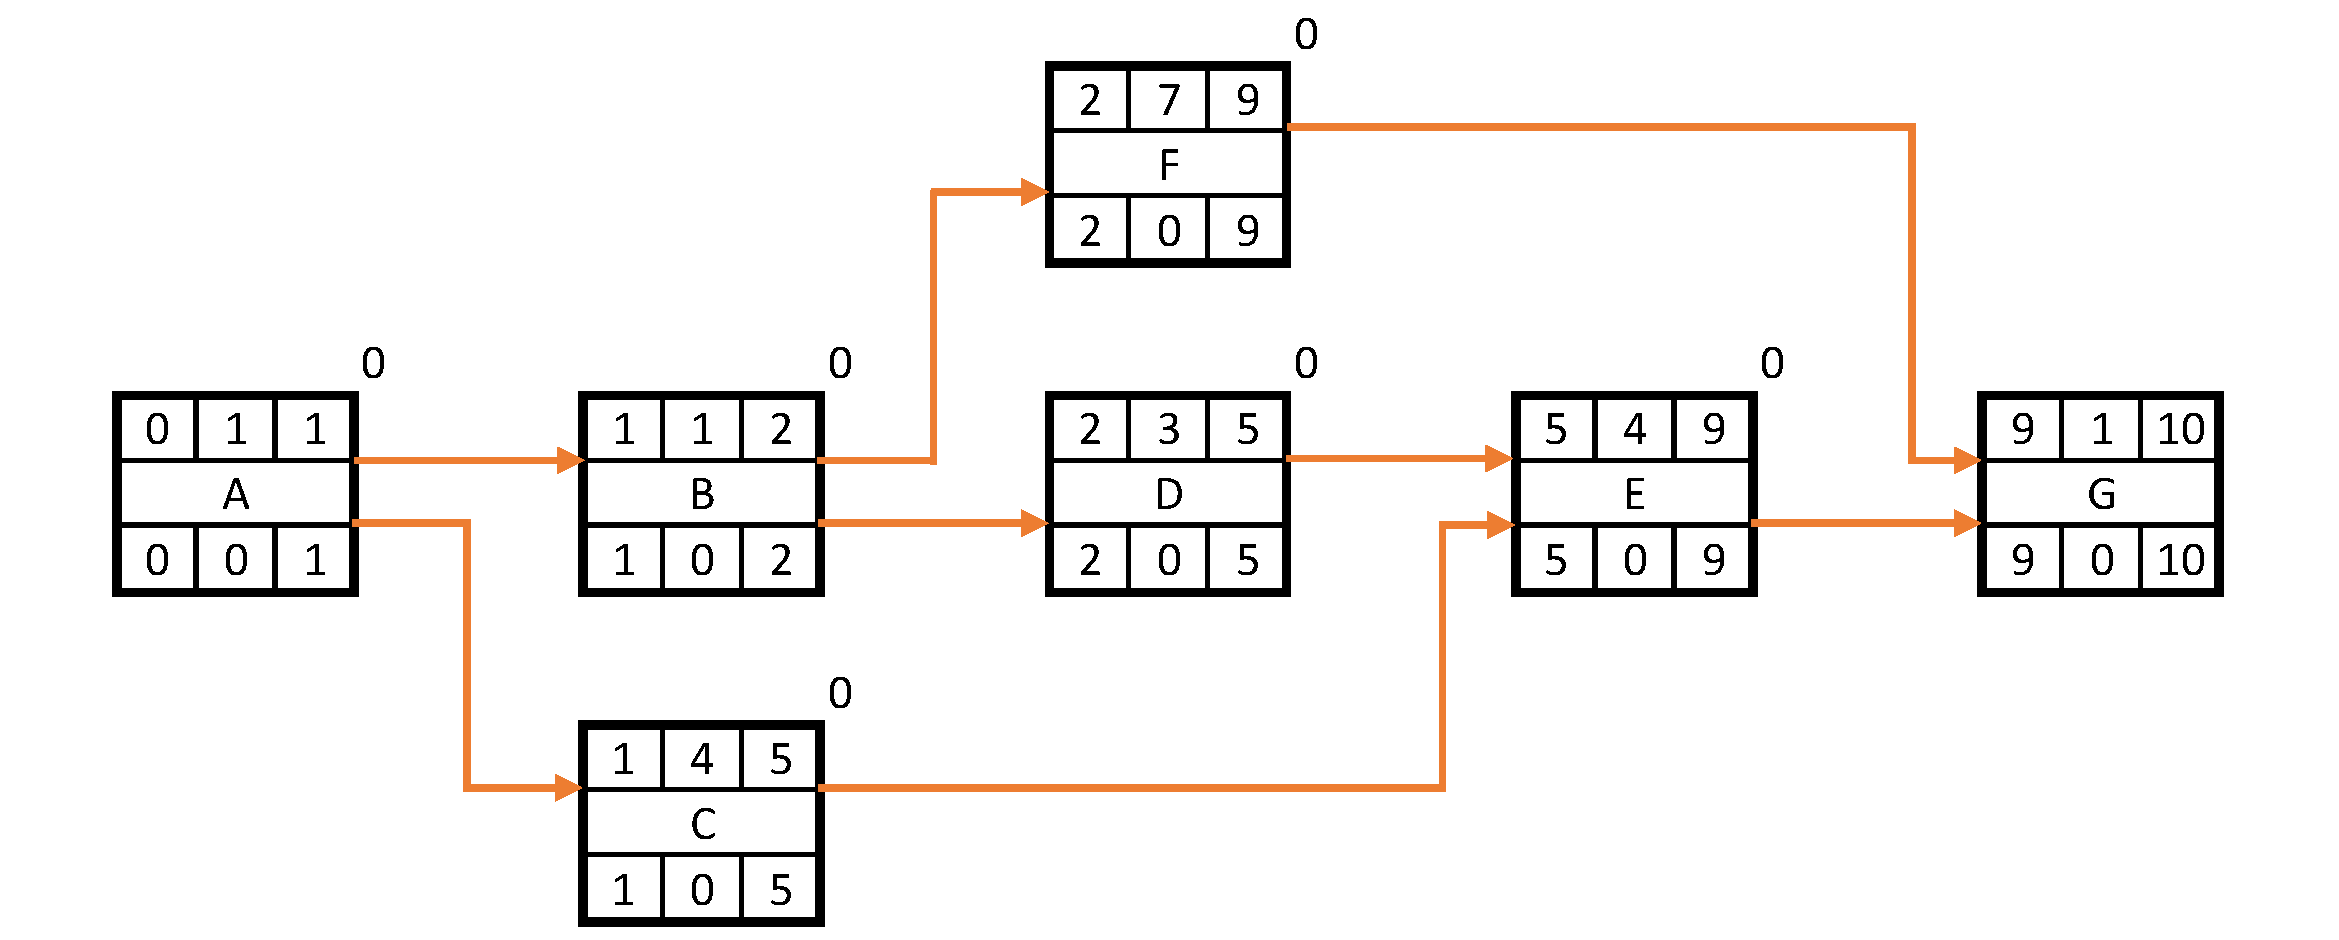
\includegraphics[width = \textwidth]{./img/qa4.png}
    \caption{Network diagram to show final project timescale.}
    \label{qa4}
\end{figure}
\end{document}